\documentclass[11pt,a4paper,oneside]{article}

\usepackage{amsmath}
\usepackage{apacite}
\usepackage{dirtytalk}
\usepackage{titlepic}
\usepackage{graphicx}
\usepackage[sort&compress,round]{natbib}
\usepackage[labelfont=bf, labelsep=period]{caption}
\usepackage[margin=3cm]{geometry}
\usepackage[english]{babel}
\usepackage{amssymb}
\usepackage{relsize}
\newcommand{\norm}[1]{\left\lVert#1\right\rVert}
\usepackage[toc,page]{appendix}


\title{
	\LARGE \textbf{Quantitative Methods} \\
	\LARGE \textbf{for the Study of Animal Behavior} \\
	\vspace{4cm}
	\Large Dissertation submitted \\
	\Large for the academic degree of \\
	\vspace{0.5cm}
	\Large \textit{Doctor of Natural Sciences} \\

	\vspace{2cm}
    \Large Presented by \\
    \vspace{0.5cm}
    \LARGE Jacob M. Graving \\
    \vspace{0.5cm}
    \Large at the \\
    \vspace{0.1cm}
	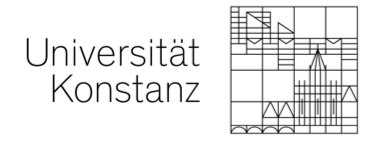
\includegraphics[width=6cm]{Graving_IMPRS_Thesis/graphics/uni_logo.png}\\
	\vspace{2cm}
	\Large Faculty of Science \\
	\Large Department of Biology \\
	\vspace{2cm}
	\Large Konstanz, 2020
	\date{}
}

\begin{document}
	\maketitle
	\pagenumbering{gobble}
    \newpage
	\tableofcontents
	\pagenumbering{roman}
	\newpage
	\label{listoffigures}
	\listoffigures
	\newpage
	\pagenumbering{arabic}
	\section{Summary of Proposal}
	\par
	Here I propose to address core questions related to how sensory information and internal state of individuals influence the collective movement dynamics of migrating animal groups. I will use marching behavior in juvenile desert locusts (\textit{Schistocerca gregaria}) as a model system.
	
	\paragraph{I will address two broad questions:}
	\begin{enumerate}
		\item How do sensory information networks drive individual decision-making and group-level movement dynamics?
		\item How do individual differences in informational, physiological, and behavioral state influence movement dynamics? 
	\end{enumerate}

	\paragraph{Within the scope of these questions I will address the following aims:}
	\begin{enumerate}
		\item Determine how visual and tactile sensory information networks influence individual decision-making and  how individual decisions influence group-level dynamics
		\item Resolve how nutritional state influences sensory perception, individual behavior, and collective movement
		\item Understand how neurophysiological dynamics of the visual system such as sensitivity and habituation affect perception and decision-making of individuals and collectives
	\end{enumerate}
	\section{General Relevance}
	\par
	Understanding how organisms process sensory information in the brain to produce behavior is one of the most exciting scientific problems of the 21st century \citep{anderson2014competho}. More specifically, revealing the sensory and behavioral mechanisms by which animal groups successfully migrate long distances has been identified as an important scientific challenge \citep{kennedy2005don,miller2005biological}. Collective behaviors like group migration can also serve as behavioral models for the study of sensory system integration and decision-making, an unresolved core issue in neuroscience and systems biology \citep{gold2007neural}. Moreover, understanding the role of sensory processing in social animal groups can help to further explain the relationships between individual and group-level decision-making, a key challenge in the field of collective animal behavior \citep{croft2008exploring,couzin2007collective}. Previous work has shown that the inclusion of sensory information in models describing collective behavior has vastly improved our ability to predict information flow through groups and collective decision-making \citep{bazazi2008collective,strandburg2013visual,strandburg2017habitat,rosenthal2015network,twomey2016vision}, yet questions related to how sensory information drives these seemingly complex phenomena remain predominantly unexplored.
	\par
	Beyond the purely biological motivations for understanding how and why animal groups behave the way they do, it is important to recall that animal groups play a major role in human agriculture and industry. For example, honeybees are key pollinators for crops, and understanding honeybee social behavior may be critical to successfully maintaining their declining populations \citep{vanbergen2013threats}. Locusts, on the other hand, are insatiable crop consumers, and understanding the rules governing their dramatic density-dependent transition from solitary to social  \citep{simpson2001gregarious} as well as the dynamics of their collective movement \citep{buhl2006disorder} and long-distance migration patterns \citep{kennedy1951migration} is an important part of managing them as an agricultural pest. In fact, it has been estimated that plagues of mass migrating insects, like locusts, impact the livelihood of one in ten people on the planet \citep{kennedy1985migration}. These are just two of many examples of how collective behavior, and insect collective behavior in particular, can have important effects on the lives of humans. 
	\par
	In addition to being important agricultural species, insects like honeybees and locusts are especially well suited as models for studying behavior due to their relatively simple neural architecture---a million or less neurons vs. tens of millions or billions in most vertebrates---and large repertoires of complex, plastic, and ecologically relevant behaviors \citep{haberkern2016studying}. Few other taxa can compete with insects as models of sensory processing and behavior as more than 100 years of research on neurobiology and behavior in ants, bees, flies, cockroaches, and locusts has generated a massive amount of genetic and neuroanatomical data, experimental protocols, and perceptual models \citep{menzel1983neurobiology,burrows1996neurobiology,feany2000drosophila,chittka2006recognition,north2007invertebrate,leonard2014multisensory,haberkern2016studying}. This uniquely positions insects at the forefront for advancing our understanding of the relationships between sensory perception and behavior.
	\par
	Despite the advantages insect model systems provide, there still exist major methodological limitations in collecting neurobiological data in freely behaving animals, and this has only recently been accomplished in a few, limited contexts (e.g. \citealp{martin2015central}). Additionally, the roles of specific neural substrates in different behavioral tasks remain ambiguous. However, computational modeling and information-theoretic approaches can help bridge the gap between sensory input and behavioral output by relating the computational requirements of a given task to the cognitive machinery offered by the brain and types of locomotion an animal can produce \citep{webb2016neural}. Such models have already provided insight into the sensory and cognitive processing required to reduce the high-dimensional, time-varying complexity of a visual scene into coordinated behavioral output (e.g. \citealp{bertrand2015bio,mischiati2015internal}). Moreover, recent advances in machine learning and information-theoretic methods are able to affirm and make precise key behavioral hypotheses through rigorous, data-driven approaches \citep{berman2014drosopholid,berman2014mapping,berman2016predictability,klibaite2017unsupervised,todd2017exploration,wiltschko2015,twomey2016vision}. Importantly, these frameworks allow researchers to address precise biological questions about the dynamics, functional consequences, and subsequent evolution of behavior. 
	\par
	During the course of my PhD, I propose to examine the interacting roles of sensory information and internal state on the dynamics of individual and collective behavior. Using machine learning and information-theoretic methods, I plan to test key assumptions about the behavior of locust swarms through rigorous, data-driven approaches. The results from these projects will provide new understanding of how locust swarms are formed and maintained over time and will inform next-generation behavioral models for predicting and preventing future outbreaks of locust plagues.

	\section{Project Description}
	\subsection[Sensory Information Networks]{Sensory Information Networks as Drivers of Individual Movement and Group Migration} \label{project1}
	\paragraph{Objective:} 
	Use computational methods to precisely understand the sensory and behavioral mechanisms driving individual decision-making and group movement
	\subsubsection{Background}

	Sensory information networks mediate the coordinated group movements of schooling fish, flocking birds, and swarming insects \citep{couzin2007collective,bazazi2008collective,strandburg2013visual,strandburg2017habitat,rosenthal2015network}, and revealing the networks underlying these group dynamics is a core issue in the study of collective behavior \citep{croft2008exploring,couzin2007collective}. In nutrient-deprived conditions, cannibalism drives the ordered movement of marching juvenile locusts. Under such conditions, individuals make movement decisions based on the threat of being cannibalized from behind and the motivation to cannibalize others ahead \citep{bazazi2008collective,romanczuk2009collective,bazazi2011nutritional,guttal2012cannibalism}. The movement of individuals within these marching bands generates social information in the form of \textit{sensory cues}. Others in the group perceive these cues and use this information to make movement decisions. These cues are \textit{multimodal}, consisting of both a visual component---the motion of nearby neighbors impinging on the retina---and a tactile component---aggressive touching and biting of the abdomen and other body parts \citep{bazazi2008collective}. These separate channels provide individuals with information about their neighbors, which they presumably \textit{integrate} when making movement decisions. 
	\par
	Both visual and tactile information play important roles in locust marching behavior. For example, blocking the forward or rear visual field with black acrylic paint reduces group movement, and blocking the rear visual field produces similar effects to blocking the \textit{entire} visual field \citep{bazazi2008collective}. In addition to vision, tactile information is an important driver of marching behavior. For example, denervating the abdomen increases rates of cannibalism and decreases group movement. Additionally, tactile activation of immobile locusts is mediated specifically through abdominal contact and  not lateral or anterior contact. Moreover, denervating the abdomen has nearly identical effects on group movement to blocking the rear visual field \citep{bazazi2008collective}. The similarity of these effects suggests that these modes of information are comparable in their level of importance and may provide individuals with information \textit{redundancy} and \textit{degeneracy}, a key hypothesis in the study of multimodal decision-making \citep{hebets2016systems,stein2012new}. Presumably individuals with denervated abdomens are less capable of detecting and escaping from neighbors trying to cannibalize them. This decreased detection ability suggests that visual information is insufficient, and to successfully avoid being cannibalized, tactile information is necessary.
	\par
	In the past, visual and tactile information channels have been studied separately, in a unimodal context \citep{bazazi2008collective}, but their combined, multimodal influence on decision-making remains uninvestigated. Additionally, due to methodological limitations, previous work on this topic has primarily examined the influence of these sensory modalities on group-level movement and not on the movement decisions of individuals. This work also relied on rather crude manipulation of the sensory systems involved. Furthermore, it is still unclear what visual features individuals attend to and what rules they follow when making movement decisions. Here I propose to investigate the dynamics of how individuals integrate multimodal information channels for decision-making and subsequently how individual decisions influence group-level movement through multimodal information networks. Rather than directly manipulating the sensory systems of individuals I will instead directly measure sensory inputs and map the relationship between sensory inputs and behavioral outputs. I will then describe the collective dynamics of locust swarms at both the individual and network level. 
	
\begin{figure}
	\begin{center}
		\includegraphics[width=\textwidth]{berman2014figure.jpg}\\
	\end{center}
	\begin{flushleft}
		\caption{An overview of the behavioral analysis framework (reproduced from \citealp{berman2014drosopholid,berman2014mapping}) \label{fig:berman2014}} 
	\end{flushleft}
\end{figure} 

	\subsubsection{Methods} \label{sec:methods}
	
	This is the primary project for my PhD thesis, and these methods will be used for all other projects. For a more detailed description of the methods, see \textit{Appendices}.
	
	\paragraph{Quantifying Perception and Behavior}
	\par
	Most previous methods for quantifying animal behavior can be placed into one of two categories. The first is to use coarse measures of locomotion such as velocity, turning, etc., or counting the number of discrete events imposed by the experimental setup, such as choosing the left or right arm of a maze. The second is to manually label data with behavioral categories determined by a human observer, and more recently, to use these labels in combination with detailed movement data and supervised machine learning classifiers to subsequently label much larger data sets \citep{kain2013leg,kabra2013jaaba}. 
	\par
	While this second method has improved the level of detail with which behavior can be measured, it is prone to researcher bias and the subjective definitions of what constitutes a behavioral \say{category}. Moreover, these methods are incapable of labeling behaviors not specified by the researcher and fail to first demonstrate from the data whether or not the behaviors can be meaningfully categorized at all. Recent advances in unsupervised machine learning methods now allow for the detailed measurement of behavior without this subjectivity \citep{berman2014drosopholid, berman2014mapping, berman2016predictability, klibaite2017unsupervised, wiltschko2015,todd2017exploration}. As previously mentioned, these methods derive a behavioral description directly from data with clearly stated assumptions and testable consequences.
	\par
	Here I propose to extend the framework proposed by \cite{berman2014mapping,berman2014drosopholid} to measure the perception and behavior of individuals within groups of animals (Figure \ref{fig:berman2014}). The basis of this approach is to view behavior as a trajectory through a high-dimensional space of postural dynamics where repeatable, sustained pauses in behavioral space indicate stereotyped behaviors while rapid movements through space correspond to non-stereotyped actions. In brief, this framework takes a video of an individual animal, rotationally and translationally aligns each frame (Appendix \ref{sec:imageregistration}), linearly compresses the dimensionality of each frame into a low-dimensional description of posture (Appendix \ref{sec:posturaldecomposition}), transforms the postural time-series to the frequency domain using a continuous wavelet transform (Appendix \ref{sec:spectrogramgeneration}), and then nonlinearly embeds each time point into a two-dimensional map (Appendix \ref{sec:spatialembedding}). The underlying probability distribution of the behavioral space is then estimated with 2-D kernel density estimation. The peaks of this probability density estimate can then be spatially segmented, using a watershed transform \citep{roerdink2000watershed}, into discrete regions of stereotyped behavior. The output of this pipeline provides a rich description of an animal's entire behavioral repertoire while respecting the underlying topology of the data at every step.
	\par
	To improve the overall computational tractability for measuring the behavior of animal groups, I have reformulated the methods introduced by \citet{berman2014mapping,berman2014drosopholid} to fit within the framework of \textit{artificial neural networks} (ANNs; Appendix \ref{sec:anns}). Reimplementing this framework as ANNs allows for highly reproducible results with learned parametric models, which after training, can be used to easily analyze new data. Importantly, most of the computation has been moved from the CPU to the GPU, which allows for highly-parallel processing and drastically reduced computation time. Moreover, I am working to further extend this framework by incorporating the direct estimation of sensory inputs to the visual system---using a ray-casting algorithm similar to software previously developed by Colin Twomey \citep{strandburg2013visual,rosenthal2015network,twomey2016vision}--- and the automatic detection of physical interactions between individuals. I will then be able to directly map, from physics first principles, the relationship between sensory inputs and behavioral outputs (Figure \ref{fig:perceptionbehavior}) in a highly rigorous and detailed way. Building on this framework, I will then be able to examine the collective dynamics of locust swarms at both the individual and network level. 
	
	\begin{figure}
		\begin{center}
			\includegraphics[width=0.8\textwidth]{perceptionbehaviorfigure.png}\\
		\end{center}
		\begin{flushleft}
			\caption{Visual field reconstruction (\textbf{left}) will be mapped to detailed behavioral output (\textbf{right}), represented here as pixel variance.\label{fig:perceptionbehavior}} 
		\end{flushleft}
	\end{figure} 
	
	\paragraph{Individual Tracking}
	A key challenge of using computer vision for quantifying collective animal behavior is the ability to track individuals over long periods of time while maintaining identities. For unmarked animals this has been solved in a number of ways \citep{perez2014idtracker,rodriquez2017toxtrac,rasch2016closing}, but typically these methods are limited to a dozen or so individuals either due to the computational complexity of the algorithms they rely on or a lack of differences in coloration that makes individual identification unreliable. Additionally, most of these methods can only be used under ideal laboratory conditions and may require extensive manual linking of trajectories (e.g. \citealp{rosenthal2015network}).
	\par
	An obvious solution for tracking larger groups is to mark individuals in a way to makes them easily distinguishable to computer vision algorithms. Examples of these markings include painting or injecting colored elastomer under the skin of each animal to create known color variation. A simpler marker solution is to attach a 2-D barcode tag to each animal. Each of these barcodes is encoded with a unique identity matrix that is some specified distance (number of bits) from all other barcodes. While attaching these markers is not tractable for many animal species, this tracking paradigm has been employed in a number of previous studies involving insects \citep{crall2016social,heyman2017ants,mersch2013tracking}.
	\par
	Here I employ my own software for tracking 2-D barcode tags inspired by \citet{crall2015beetag}. This software is greatly improved over other barcode tracking implementations in terms of both speed and accuracy. The software provides a high-level Python API for the automated measurement of animal behavior and locomotion, and it is currently being used internally at the Max Planck Institute for Ornithology. This software is quickly becoming a standard tool for the study of collective and social behavior in a variety of species (Figure \ref{fig:barcodefigure}), and I plan to make the source code publicly available after publication.
	\par
	Locusts are generally robust to physical manipulation, including invasive surgery \citep{bazazi2008collective}; therefore, we are able to directly attach these markers to individuals, using cyanoacrylate glue, without issue. The tracking problem is then greatly simplified (Figure \ref{fig:locustbarcodefigure}). While this method relies on the barcode to be visible for successful tracking, missing trajectory data caused by occlusions can be inferred using interpolation for small gaps or basic object tracking algorithms for longer spans of missing data. 
	

	\begin{figure}
		\begin{center}
			\includegraphics[width=1\textwidth]{barcodefigure.png}\\
		\end{center}
		\begin{flushleft}
			\caption{Barcodes being used to track African cichlids (\textbf{top-left} and \textbf{bottom-right}), sunbleak (\textbf{bottom-left}) and zebrafinches (\textbf{top-right}). This technology gives detailed insight into the subtle social interactions driving collective behavior (\textbf{bottom}).\label{fig:barcodefigure}} 
		\end{flushleft}
	\end{figure} 
	
	\begin{figure}
		\begin{center}
			\includegraphics[height=0.90\textheight]{locustbarcodefigure.png}\\
		\end{center}
		\begin{flushleft}
			\caption{Barcodes are used to track locusts (\textbf{top}) and generate trajectories for each individual (\textbf{bottom}) while maintaining identity (colored lines).\label{fig:locustbarcodefigure}} 
		\end{flushleft}
	\end{figure} 

	\paragraph{Experimental Setup}
	I will conduct experiments in white, plastic behavioral arenas similar to \citet{buhl2006disorder,bazazi2008collective,bazazi2011nutritional} (see Figure \ref{fig:locustbarcodefigure}). The arenas will be filmed in a climate-controlled room using a high-resolution (2048$\times$2048px, 90Hz or 4112$\times$3008px, 31Hz), monochrome machine vision cameras.

	\paragraph{Current State}
	The barcode tracking, behavioral classification, and visual field reconstruction software packages are all near completion. The experimental setup has been constructed. Preliminary experiments have been completed. Final experiments are planned for August-December 2017.
	
	\subsubsection{Timeline}
	\begin{itemize}{}{}
		\item Project duration --- 2.5 years
		\item Software development --- 1.5 years
		\item Construction of experimental setup --- 4 months
		\item Obtaining preliminary results --- 2 months
		\item Obtaining final results --- 4 months	
		\item Final discussions and writing up --- 2 months.
	\end{itemize}
	

\subsection[Nutritional State and Sensory Perception]{The Influence of Nutritional State on Sensory Perception and Group Movement} \label{project2}
\paragraph{Objective:} 
Resolve how nutritional state influences individual sensory perception, decision-making, and group movement
\subsubsection{Background}
Nutritional state can drastically influence the behavior of individuals in groups \citep{lihoreau2015nutritional}. For example, individuals with the highest nutrient requirements are more likely to lead groups \citep{krause1992relationship,fischhoff2007social,mcclure2011group}. In schools of roaches (\textit{Rutilus rutilus}), unfed individuals tend to take front positions \citep{krause1992relationship}, and this position in the group provides them with the highest food intake and a dominant influence on directional decisions of the group \citep{bumann1993front}. In the nomadic forest tent caterpillar (\textit{Malacosoma disstria}), the most protein-deficient individuals initiate collective foraging and lead the group towards new feeding sites, whereas protein-satiated individuals follow behind \citep{mcclure2011group}. Differences in nutritional state among individuals can regulate the emergence of \textit{temporary leadership roles}, where a single individual can determine the movement decisions of the entire group \citep{sumpter2010collective}. 
\par
Nutritional state can also influence sensory perception. For example, when deprived of food, blowflies (\textit{Calliphoridae sp.}) will downregulate activity in their peripheral visual system---presumably to reduce the costs of an energetically expensive sensory system---and increase reliance on energetically cheaper sensory modalities such as olfaction \citep{longden2014nutritional}. Similar changes have been demonstrated in vertebrates as well (reviewed by \citealp{longden2014nutritional}). Additionally, a key assumption of animal communication theory is that receivers dynamically alter their perceptual rules for weighting information modalities depending on relevance, context, and internal state \citep{hebets2016systems}---commonly referred to as \textit{cross-modal perceptual weighting} \citep{stein2012new}, but this assumption is rarely tested explicitly with few notable exceptions (e.g. \citealp{gomes2016bats}).
\par
While the behavioral effects of nutritional state have been studied in locusts \citep{bazazi2011nutritional}, the interacting effects of nutritional state and sensory information have not. \citet{bazazi2011nutritional} showed that protein-deprived locusts move faster when in groups with increased rates of cannibalism, and supplementing locusts with a high-protein diet decreases group movement \citep{bazazi2011nutritional}. However, this study only examined groups with homogeneous nutritional states, and the dynamics of heterogeneous groups remain unstudied. Within heterogenous groups, nutrient-replete individuals should be better able to escape those trying to cannibalize them, as larger energy reserves allow them to move faster for longer \citep{arrese2010insect}. These pursuit and escape responses are mediated by multimodal sensory networks \citep{bazazi2008collective}, and the magnitude, frequency, and modality of sensory stimuli within these networks are a product of other group members' behavior. Movement in response to these sensory stimuli can also influence nutritional state, as faster moving individuals expend more energy, quickly returning to a state of nutrient-deprivation \citep{arrese2010insect} and increasing their motivation to cannibalize others. These heterogeneous autocatalytic dynamics may be comparable to the dynamics of other complex systems (e.g. \citealp{ortega2016visualization,bissette2013mechanisms})
\par
For the sake of theoretical tractability, models of locust marching behavior have also not explicitly, comprehensively, and simultaneously considered many related aspects that may be driving collective movement in locust bands \citep{guttal2012cannibalism,bazazi2011nutritional,romanczuk2009collective}. These aspects include the role of nutritional state in altering the perception and behavior of individuals, the role of individual behavior in altering the movement of others in the group through sensory interaction networks, the role of locomotion in altering nutritional state, and the feedback between these factors and the environment, e.g. the distribution of food resources. Consequently, there exists only a meager theoretical basis for understanding these dynamics.
\par
Past research offers limited understanding of how differences in nutritional state can alter perception, behavior, and the dynamics of group movement. Nutritionally-driven behavioral differences \citep{bazazi2011nutritional} presumably change the magnitude and frequency of visual and tactile interactions between individuals, and while it has been shown that nutritional state alters the decision-making of individuals, it is not precisely understood how these nutritional differences alter sensory perception and internal decision-making rules. None of these questions have been tested explicitly, and here I propose to do so for the first time.


\subsubsection{Methods}

See \ref{sec:methods} for description of experimental setup and general methods.

\paragraph{Experimental Diets}
I will use artificial diets described by Bazazi et al. (2011) to manipulate the nutritional state of individuals. Treatment groups will consist of different mixtures of individuals fed on high- and low-nutrient diets. The exact experimental design will be determined after completion of  \ref{project1} and pilot experiments for \ref{project2}.

\paragraph{Data Analysis}
I will use previously described methods (see \ref{sec:methods}) to compare the perception and behavior of nutritionally-deprived individuals to nutritionally-replete individuals. I will then relate this to the dynamics of collective movement.

\paragraph{Current State}
The barcode tracking, behavioral classification, and visual field reconstruction software packages are all near completion. The experimental setup has been constructed. Final experiments are planned for early 2018.

\subsubsection{Timeline}
\begin{itemize}{}{}
	\item Project duration --- 6 months
	\item Obtaining preliminary results --- 2 months
	\item Obtaining final results --- 2 months	
	\item Final discussion and writing up --- 2 months.
\end{itemize}

\subsection{The Neurobehavioral Dynamics of Group Movement}
\paragraph{Objective:} 
Describe the neurobiological implementation of visually-mediated behavioral programs in locusts and understand how neurophysiological dynamics, such as sensitivity and habituation, affect perception and decision-making of both individuals and collectives.
\subsubsection{Background}
Based on neurophysiology \citep{rind2008arousal,rogers2010spatiotemporal}, loom stimuli created by movement of conspecifics likely contribute significantly to locust marching behavior (reviewed by \citealp{simmons2010escapes}). The largest neurons in locust visual system, the descending contralateral movement detector (DCMD) and lobula giant movement detector (LGMD) (Figure \ref{fig:dcmd}), are highly sensitive to loom stimuli, and there is strong evidence that these neurons are involved in social behaviors. These pathways mediate object avoidance \citep{chan2013collision,gabbiani2002multiplicative} and their activity has been linked to a wide range of collision avoidance behaviors during flight \citep{simmons2010escapes}. Habituation of DCMD to loom stimuli is also five times weaker in gregarious locusts than in solitary locusts \citep{matheson2004plasticity} suggesting that signal transduction by this neuron may be important for social interactions. However, the exact neurophysiological mechanisms of how locusts make decisions in a social context remain almost completely unstudied.
\par
Previous neurophysiological studies of the locust visual system have been primarily limited to tethered experiments with arbitrary visual cues chosen a priori. Instead of making assumptions about which sensory features are relevant to social behavior, I will work backwards by directly immersing a freely behaving locust into a real social context while recording neurophysiological data from the visual system. I will then measure the visual inputs and behavioral outputs using computer vision. Using machine learning methods, I will decompose the relevant visual features, map these features to the features of the recorded neural encoding and map the neural encoding to the behavioral output. This will be the first time all three of these aspects are considered in such a detailed, comprehensive manner and in an ecologically-relevant context. This project will provide new understanding of neurophysiological dynamics of both collective behavior and animal behavior in general.

\subsubsection{Methods}

See \ref{sec:methods} for description of experimental setup and general methods.
\begin{figure}
	\begin{center}
		\includegraphics[width=0.5\textwidth]{dcmdfigure.png}\\
	\end{center}
	\begin{flushleft}
		\caption{In collaboration with others, I will record from the DCMD (\textbf{top}) via the neck connectives (\textbf{bottom}). Figures reproduced from \citealp{berman2013neural,gabbiani2002multiplicative}.  \label{fig:dcmd}} 
	\end{flushleft}
\end{figure} 

\begin{figure}
	\begin{center}
		\includegraphics[width=\textwidth]{electrophysiologyfigure.png}\\
	\end{center}
	\begin{flushleft}
		\caption{Spike sorting using unsupervised machine learning. To better understand how the brain encodes visual information, I have developed software for analyzing electrophysiology traces (\textbf{A}) by automatic spike sorting. Spikes with an amplitude above an automatically determined noise threshold (blue dashed line) are extracted (red spikes, \textbf{B}), embedded into a low-dimensional space (using t-SNE) based on shape (\textbf{C}) and then labeled based on automatic cluster assignment (\textbf{D}) using DBSCAN \citep{ester1996density}. \label{fig:ephys}} 
	\end{flushleft}
\end{figure} 

\paragraph{Neurophysiology}
Collaborating with members of the neurobiology department, I will record from the DCMD via the neck connectives (see \citealp{williamson1982large,berman2013neural} for details) of freely moving locusts interacting with a social group. I will track individual behavior in detail and reconstruct the visual field using the software previously described in \ref{sec:methods}. 

\paragraph{Data Analysis}
Using similar machine learning methods from \ref{sec:methods}, I will relate the visual field to the neural encoding and then relate the neural encoding to the behavioral output (see Figure \ref{fig:ephys} for details).

\paragraph{Current State}
The barcode tracking, behavioral classification, and visual field reconstruction software packages are all near completion. Software for analyzing the electrophysiology data is in development (Figure \ref{fig:ephys}). The experimental setup has been constructed. Electrophysiology rig has been purchased and set up. Recording methods are in development by Angela Albi (PhD student) and Einat Couzin (Principle Investigator). Final experiments are planned for late 2017 - early 2018 depending on the progress with neurophysiology recordings.

\subsubsection{Timeline}
\begin{itemize}{}{}
	\item Project duration --- 6 months
	\item Obtaining preliminary results --- 2 months
	\item Obtaining final results --- 2 months	
	\item Final discussions and writing up --- 2 months.
\end{itemize}


\section{Additional PhD Curriculum}
\subsection{Workshops}
\paragraph{Attended:}
\begin{itemize}
	\item IMPRS Student Retreat 2015
	\item Social Network Analysis
	\item Conference Presentations
	\item Teaching Week
	\item Introduction to GAM and GAMM with R
	\item IMPRS Student Retreat 2016
	\item Introduction to Scientific Writing
\end{itemize}
\paragraph{Plan to Attend:}
\begin{itemize}
	\item Writing Lab for Research Articles
	\item Grant Writing
\end{itemize}
\subsection{Conferences and Symposia}
\paragraph{Attended:}
\begin{itemize}
	\item IMPRS Grand Challenges Symposium 2015: Scientific Communication - Seewiesen, Germany
	\item IMPRS Grand Challenges Symposium 2016: Evolutionary Ecology of Individual Differences - Konstanz, Germany
	\item IMPRS Selection Symposium 2016 - Seewiesen and Konstanz, Germany
	\item European Conference for Behavioural Biology 2016 - Vienna, Austria
	\item ImVis 2017 - Faak am See, Austria
\end{itemize}
\paragraph{Plan to Attend:}
\begin{itemize}
	\item DeepLearn2017 - Bilbao, Spain
\end{itemize}
\subsection{Public Outreach}
\paragraph{Attended:}
\begin{itemize}
	\item Volunteered at \say{Das Schwarmverhalten der Fische}, a public lecture given by Prof. Dr. Jens Krause in Konstanz, Germany
	\item Volunteered at \say{Konstanzer Lange Nacht der Wissenschaften}
\end{itemize}
\paragraph{Plan to Attend:}
\begin{itemize}
	\item Any future scientific communication events organized by the department 
\end{itemize}
\pagebreak


\begin{appendices}
\pagenumbering{roman}
\begin{figure}
	\begin{center}
		\includegraphics[width=0.3\textwidth]{neuralnetwork.png}\\
	\end{center}
	\begin{flushleft}
		\caption{A simple feed-forward neural network. \label{fig:feedforward}} 
	\end{flushleft}
\end{figure} 

\section{Artificial Neural Networks}  \label{sec:anns}
Artificial neural networks (ANNs) are a class of computational model loosely inspired by biological neural networks in the brain. These models rely on the metaphor of a \textit{computational graph} where a network is represented by a series of interconnected computational \textit{nodes}, also called \textit{neurons}, which form the \textit{layers} of the computational graph. In the simple case of a feed-forward neural network $f: X \to Y$, there is an \textit{input layer} where data $X$ are fed into the network and an \textit{output layer} where the computational output of the network $\hat{Y}$---an estimate of the ground truth $Y$---is produced, and these are connected by one or more \textit{hidden layers} (Figure \ref{fig:feedforward}). As a side note, ANNs are sometimes called \textit{deep neural networks} (DNNs) depending on how many layers of computational nodes they contain, where a network with more than 2 hidden layers is considered \textit{deep}. These hidden layers make up the computational functionality of the graph, with each node of the layer containing parameters known as \textit{weights} and \textit{biases}. Typically the weights and biases of each layer are denoted as a matrix $W^l$ and a vector $\mathbf{b}^l$ respectively, where $l$ is the layer number. At the output of each layer is a function that uses the weights and biases to perform some computation, typically called an \textit{activation}. The activations for the first two hidden layers of a feed-forward ANN are therefore denoted by
\begin{equation}
\begin{aligned}
& \mathbf{a}^1 = h^{1}(W^1\mathbf{x} + \mathbf{b}^1)  \qquad \text{and}\\
& \mathbf{a}^2 = h^{2}(W^2\mathbf{a}^1 + \mathbf{b}^2)\\
& \quad \equiv h^2(W^2h^1(W^1\mathbf{x} + \mathbf{b}^1) + \mathbf{b}^2) 
\end{aligned}
\end{equation}
where $\mathbf{x} \in X$ is the input, and $h^{l}(\cdot)$ is some activation function for layer $l$ (linear, sigmoid, or otherwise). 
\par
The cost function for optimizing these parameters is defined as 
\begin{equation}
C = C(Y,\hat{Y})
\end{equation}
where $C$ is some function penalizing the network output $\hat{Y}$ for being different from the ground truth $Y$. This cost function is then typically minimized, or rather the network is \textit{trained}, through a modified version of gradient descent known as \textit{mini-batch stochastic gradient descent with backpropagation}. In brief, this process is performed in three steps: (1) mini-batches of training data are fed through the network in a forward pass, (2) the error of the output is calculated, and (3) the gradients $\frac{\delta C}{\delta W}$ and $\frac{\delta C}{\delta \textbf{b}}$ are propagated backwards sequentially through the network using the chain rule, updating the parameters $W^l$ and $\mathbf{b}^l$ at each layer $l$. The cost function in the context of this optimization algorithm then takes the form
\begin{equation}
C = \frac{1}{n} \sum_{i=1}^{n} C_i \text{,}
\end{equation}
where $C$ is the average for all cost functions $C_i$ for all $n$ training examples.  
\par
These networks are highly flexible and can be used for everything from image segmentation, object tracking, classification, regression, time-series modeling, and in this case, dimensionality reduction \citep{deeplearningbook}. In fact, there is evidence they can be used to approximate nearly any function or probability distribution \citep{lin2016does}.




\section{Image Registration} \label{sec:imageregistration}
Using the barcode tracking data described in the main text, following \citet{berman2014mapping,berman2014drosopholid} I first generate 200$\times$200px videos of each individual over time. This is accomplished by segmenting the animal from the background and rotationally and translationally aligning each frame to a basis image such that the main trunk of the body is mostly invariant while the limbs are allowed to vary (Figure \ref{fig:alignment}). The details of these alignment algorithms are described elsewhere \citep{berman2014drosopholid,berman2014mapping,de1987registration,reddy1996fft,wilson2006correlation,guizar2008efficient}. Because these images are not lit from behind like the methods described in \citet{berman2014drosopholid,berman2014mapping}, individual color variation can influence the results of the analysis. To solve this, I simply binarize each image such that the pixels describing the body of the animal are white, while the background pixels are black (Figure \ref{fig:convexhull}). 
\par To isolate the pixels describing the behavior of one individual from those describing the behavior of other individuals, I use only those pixels within the convex hull of the pixels with the highest variance (see Figure \ref{fig:convexhull}). This provides a reasonable representation of individual behavior but is still problematic when animals are in very close proximity. This issue has been adequately solved by \citet{klibaite2017unsupervised} for cases where there are only two interacting animals, but this method is unreliable when there are more than two animals interacting. I am currently investigating the use of \textit{fully convolutional neural networks}, a class of ANNs designed for image segmentation \citep{long2015fully}, to produce a higher-quality solution to this problem. After all of these steps, I then utilize these videos as a high-dimensional time-series describing the posture of each individual with a single frame being a feature vector describing the pose at time point $t$, or 
\begin{equation}
X \equiv \{x_1(t),x_2(t),\ldots,x_d(t)\} \text{,}
\end{equation}
where $d$ is the dimensionality of the images. 


\begin{figure}
	\begin{center}
		\includegraphics[width=0.6\textwidth]{alignmentfigure.png}\\
	\end{center}
	\begin{flushleft}
		\caption{The image alignment algorithm. Images are roughly aligned using the vector angle generated from reading the barcode (\textbf{top-left}), segmented from the background such that only the body trunk and rear legs are visible (\textbf{bottom-left}) and then aligned (\textbf{bottom-right}) with a basis image (\textbf{top-right}).  \label{fig:alignment}} 
	\end{flushleft}
\end{figure} 

\begin{figure}
	\begin{center}
		\includegraphics[width=0.8\textwidth]{convexhullfigure.png}\\
	\end{center}
	\begin{flushleft}
		\caption{The convex hull (\textbf{middle}) of high variance pixels (\textbf{left}) used to segment pixels for measuring individual behavior (\textbf{right}).  \label{fig:convexhull}} 
	\end{flushleft}
\end{figure} 



\section{Postural Decomposition} \label{sec:posturaldecomposition}
\paragraph{}
As an insect is composed of a relatively inflexible body segments connected by mobile joints, the number of postural degrees of freedom is much smaller than the current high-dimensional image representation. Following \cite{berman2014mapping,berman2014drosopholid} I then wish to compress this representation to a lower dimensional space while still adequately describing the information contained in the high-dimensional space. \cite{berman2014mapping,berman2014drosopholid} use principal components analysis (PCA) to reduce the dimensionality of images by decomposing the covariance of pixel values into linearly uncorrelated eigenmodes. However, using PCA on large, high-dimensional data sets becomes computationally intractable due to the complexity of the underlying algorithm $O(d^2n+d^3)$, where $d$ is the number of dimensions and $n$ is the number of rows in the data matrix. There are solutions to this problem other than vanilla PCA (e.g. \citealp{rokhlin2009randomized,artac2002incremental}), but these do not provide the flexibility of an ANN and are generally difficult to implement on the GPU. 
\par
Therefore, I have reformulated this step of the framework as an ANN known as a \textit{linear autoencoder}. This implementation has multiple advantages compared to PCA, the most important of which is the ability to train the network online, or out-of-memory, on a GPU using batches of data. Because of this, the overall complexity of the algorithm reduces to low-order polynomial time \citep{magdon2015}. This also allows us to simplify the methods described in \cite{berman2014drosopholid,berman2014mapping}, as we can skip the steps of converting the images to radon space and using only pixel values with the highest variance. Instead, we can directly decompose the high-dimensional images to a low-dimensional representation. 
\par 
In the most general sense, autoencoders are a class of ANNs that seek to copy their inputs to their outputs while minimizing information loss. Autoencoders are defined in the general form $f: X \to Z \to \hat{X}$ \citep{deeplearningbook,hinton2006autoencoder,williams1986learning}. Internally the network architecture has a hidden layer that describes a code $Z$ to represent the input. The network is composed of two parts: an encoder $g: X \to Z$ and a decoder $h: Z \to \hat{X}$ that produces a reconstruction of the input data  (Figure \ref{fig:network}A). The network is then trained to minimize

\begin{equation}
\begin{split}
C(X,\hat{X}) & = C\big(X, f(X)\big) \\
& = C\Big(X, h\big(g(X)\big)\Big) \text{,}
\end{split}
\end{equation}

where $C$ is a cost function penalizing $\hat{X}$ for being dissimilar from $X$, such as mean squared error or cross entropy.
\par
Autoencoder networks are typically designed so that this copying task will result in the encoder $g(X)$ learning some useful description of the data space $X$ rather than simply the identity, i.e. $X \neq g(X) = Z$. One way to achieve this is to create a bottleneck in the network by constraining $Z$ to a lower-dimensional space than $X$. Learning this lower-dimensional representation forces the autoencoder to capture the most important features of the data. Subsequently, when the decoder $h(Z)$ is \textit{linear} and $C$ is the \textit{mean squared error}, the encoder $g(X)$ will learn to span the same subspace as PCA, i.e.  minimizing information loss of the reconstruction $\hat{X}$ maximizes variance explained by the encoded space $Z$ \citep{deeplearningbook}. In this sense, PCA is the optimal linear autoencoder with respect to global information loss (see \citealt{magdon2015} for details). In practice, linear autoencoders can only achieve near-PCA performance, but this is adequate for my purposes. 

\par
To perform linear decomposition of rotationally and translationally aligned images, I define a feed-forward neural network $f: X \to Z \to \hat{X}$. The network is composed of an encoder $g: X \to Z$ that maps input images $X$ to the latent space $Z$ and a decoder $h: Z \to \hat{X}$ that then maps the encoding $Z$ to a reconstruction of the original image $\hat{X}$. For ease of explanation, I will temporarily relax the computational graph metaphor of a neural network. More formally, the data matrix is $X \in \mathbb{R}^{n \times d}$ (each row $x_i^{T} \in \mathbb{R}^{1 \times d}$ is a data point in $d$-dimensions). The autoencoder is then a pair of linear mappings
\begin{align}
& g: \mathbb{R}^d \mapsto \mathbb{R}^k \qquad  \text{and}\\
& h: \mathbb{R}^k \mapsto \mathbb{R}^d \text{,}
\end{align}
where $k < d$, specified by an encoder matrix $G \in \mathbb{R}^{d \times k}$ and a decoder matrix $H \in \mathbb{R}^{k \times d}	$. For each data point $\mathbf{x} \in \mathbb{R}^d$, the encoded feature vector is defined as
\begin{equation}
\mathbf{z} = g(\mathbf{x}) = G^{T}\mathbf{x} \in \mathbb{R}^k
\end{equation}
and the reconstruction is
\begin{equation}
\mathbf{\hat{x}} = h(\mathbf{z}) = H^{T}\mathbf{z} \in \mathbb{R}^d \text{.}
\end{equation}
Using $\hat{X} \in \mathbb{R}^{n \times d}$ to denote the reconstructed data matrix, I then have
\begin{equation}
\hat{X} = XGH \text{.}
\end{equation}
Returning to the neural network metaphor, the output of the autoencoder network $f: X \to Z \to \hat{X}$ is subsequently defined as
\begin{equation}
\hat{X} = XW^{l-1}W^l
\end{equation}
where $W$ is a matrix of weights for a single layer and $l$ is the total number of layers in the network ($l=2$ in this case).
Importantly, this implementation lacks any bias vectors, i.e.
\begin{equation}
\hat{X} = XW^{l-1}W^l = W^l(XW^{l-1}+\mathbf{b}^{l-1}) + \mathbf{b}^{l} \text{,}
\end{equation}
which enforces orthogonality in the latent space---a desirable property if the goal is to match the results of PCA \citep{konda2014zero}. 
\par
Because PCA is also typically performed on centered and scaled data (i.e. on the covariance or correlation matrix respectively), I also add a batch normalization, or \textit{batch norm}, layer between the input and the encoder layer. Batch norm is a layer commonly used for artificial neural networks to maintain activations at zero mean and unit variance, thereby speeding up convergence \citep{ioffe2015batch}. Here I use it to center the input data such that 
\begin{equation}
\hat{X} = \mathit{BN}_{\gamma,\beta}(X)W^{l-1}W^l \text{,}
\end{equation}
where $\mathit{BN}_{\gamma,\beta}(\cdot)$ is the batch norm function with learnable parameters $\gamma$ and $\beta$ for scale and shift respectively. The batch norm layer performs the computation
\begin{equation}
a_i = \mathit{BN}_{\gamma,\beta}(x_i)  \equiv \frac{\gamma (x_i - \mu)}{\sqrt{\sigma^2+ \epsilon}} + \beta 
\end{equation}
where $a_i$ is the output of the batch norm layer for mini-batch $x_i \in X$, $\epsilon$ is a small number added to avoid division by zero, $\mu$ is the mini-batch mean
\begin{equation}
\mu = \frac{1}{m} \sum_{i=1}^{m}x_i\text{,}
\end{equation}
 and $\sigma^2$ is the mini-batch variance
 \begin{equation}
 \sigma^2 = \frac{1}{m} \sum_{i=1}^{m}(x_i-\mu)^2 \text{.}
 \end{equation}
In this case, I am only interested in centering the data. Therefore, I parameterize the batch norm layer such that such that 
\begin{equation}
a_i = \mathit{BN}_{\beta}(x_i) \equiv x_i -  \mu + \beta  \text{.} 
\end{equation}
\par
Now that the details of the network design are clear, the cost function for training the network is defined as 
\begin{equation}
C = \mathit{MSE}(X,\hat{X}) \equiv \frac{1}{n} \sum_{i=1}^{n} \norm{\mathbf{\hat{x}}_i -\mathbf{x}_i}^2 \text{.}
\end{equation}

The minimization of the cost function $C$ can be performed, like any other feed-forward neural network, by mini-batch stochastic gradient descent with backpropagation---using any of a number of learning algorithms now commonplace in the machine learning literature (reviewed by \citealt{ruder2016}). 
\par
After training, the decoder $h(Z)$ is discarded, and the data matrix $X \in \mathbb{R}^{n\times d}$ is transformed with the encoder $g(X)$ into the latent space $Z  \in \mathbb{R}^{n\times k}$ to reduce the dimensionality from $d$ to $k$. $Z$ is then a linearly-compressed $k$-dimensional description of posture at each time point with each dimension representing a mode of variation within the postural space, or 
\begin{equation}
Z \equiv \{z_1(t),z_2(t),\ldots,z_k(t)\} \text{.}
\end{equation}

\par
The question then remains, how to set $k$ for dictating the dimensionality of the latent space. \cite{berman2014mapping,berman2014drosopholid} chose to use 50 eigenmodes based on the finite sampling error of the data, which is determined by performing PCA on a shuffled data matrix. This choice is complicated by the fact that, unlike PCA, a linear autoencoder is a sub-optimal solution for linear compression. I find that the results of the final behavioral mapping are qualitatively invariant to the choice of $k$, provided it is large enough. Since most of the intensive computation has been moved to the GPU, increasing the dimensionality of this step does not drastically affect computation time for the rest of the pipeline, but it does indeed have an effect. Currently, I am using $k=$ 200, but the effects of this hyperparameter on the quality of the final embedding need to be explored more rigorously to find an optimal value. 
\par
Unlike \citet{berman2014drosopholid,berman2014mapping} I find that parts of this compressed description are directly interpretable. By visualizing the encoder weights of each postural mode, I find that the three modes with the largest encoder weights (comparable to the first three eigenmodes from PCA) are describing postures related to typical tripod-gait locomotion as well as the positions of the rear legs corresponding to left and right turns (Figure \ref{fig:posture}). The remaining postural modes are not as easily interpretable, which is likely due to the nonlinear topology of the postural space.

\begin{figure}	
	\begin{center}
		\includegraphics[width=1\textwidth]{posturefigure.png}\\
	\end{center}
	\begin{flushleft}
		\caption{A visualization of the three postural modes with the largest encoder weights (ordered from left to right). When values for these modes are positive limbs are in the red locations, and when values are negative limbs are in the blue locations (see Figure \ref{fig:spectrogram}).\label{fig:posture}} 
	\end{flushleft}
\end{figure} 

\section{Spectrogram Generation}  \label{sec:spectrogramgeneration}
The instantaneous values of the postural modes do not provide a complete description of behavior, as the definition of stereotypy within this framework is intrinsically dynamical. Within this postural space, it is challenging to recognize behaviors that correspond to similar sequences of movements especially considering the possibility that limbs can move at different times and with different durations. To solve this, I  follow \cite{berman2014mapping,berman2014drosopholid} to generate spectrograms of the postural modes $z_k(t)$. Using a Morlet continuous wavelet transform, I calculate the power spectrum $S(k,f;t)$ for each mode $k$. I also use a dyadically-spaced set of frequencies between $f_{min} = 1$ Hz and the Nyquist frequency ($f_{max} = 45$ Hz) via
\begin{equation}
f_i = f_{max}2^{\frac{i-1}{N_{f}-1}log_2\frac{f_{max}}{f_{min}}}
\end{equation}
for $i = 1, 2, \ldots , N_f$. $S(k,f;t)$ is comprised of 25 frequencies for each of the 200 postural modes, making each point in time represented by a 5000-dimensional feature vector. The feature vector at each time point is then a description of changes in posture over multiple timescales, which will now be referred to as the postural dynamics space, or simply the behavioral space.

\begin{figure}
	\begin{center}
		\includegraphics[width=0.7\textwidth]{spectrogramfigure.png}\\
	\end{center}
	\begin{flushleft}
		\caption{A spectrogram (\textbf{top}) of the first postural mode (\textbf{bottom}), which describes locomotion related postures (see Figure \ref{fig:posture}). Note the characteristic frequency of locomotion. \label{fig:spectrogram}} 
	\end{flushleft}
\end{figure} 

\section{Spatial Embedding} \label{sec:spatialembedding}

Given that the dynamics of the behavioral space likely do not fill the current 5000-dimensional parameterization, I now seek to reduce the dimensionality of this representation in a way that preserves the local neighborhood relationships. \citet{berman2014mapping,berman2014drosopholid} use t-distributed stochastic neighbor embedding (t-SNE) to map high-dimensional behavioral feature vectors into a low-dimensional embedding as a way to capture the most important features of the dataset. Like all dimensionality reduction techniques, t-SNE maps a high-dimensional space to a low-dimensional space while preserving a set of invariants. t-SNE was chosen for this step as it reduces dimensionality by distorting the distances between more distant points while preserving distances between nearby neighbors with minimal local distortion.
\par
I have reformulated this step of the framework as a DNN known as parametric t-SNE. Similar to replacing PCA with a linear autoencoder, this reduces the computational complexity of the algorithm to low-order polynomial time. I largely follow the methods introduced by Van der Maaten and Hinton (2008) and Van der Maaten (2009)---with modifications following Berman et al. (2014)---to train a feed-forward neural network to learn the parametric mapping $f: X \to Y$ between a high-dimensional data space X and the low-dimensional latent space Y (Figure \ref{fig:network}). 
\par
To achieve this, pairwise distances $d(t_i,t_j)$ (yet undefined) are calculated between each time point $i$ and $j$. The distances are transformed into probabilities by centering an isotropic Gaussian over each time point $i$, computing the density of time point $j$, and renormalizing, yielding the conditional probabilities $p_{j|i}$
\begin{equation}
p_{j|i}= \frac{exp(-d(t_i,t_j)^2/2\sigma^2_i)}
{\sum_{k\neq i} exp(-d(t_i,t_k)^2/2\sigma^2_i)}.
\end{equation}
The conditional probabilities are then symmetrized to form a single joint distribution
\begin{equation}
p_{ij} = \frac{(p_{j|i} + p_{i|j})}{2n},
\end{equation}
and the joint probabilities $p_{ij}$ are then a measure of similarity between time points $i$ and $j$.
\par
To measure the pairwise similarity of time points $i$ and $j$ in the latent space, a symmetric distribution, which for technical reasons is a heavy-tailed Student-t distribution (van der Maaten, 2009; van der Maaten, 2008), is centered over each time point $i$ in the latent space. Again, the density of time point $j$ under this distribution is measured and the result is renormalized to obtain joint probabilities $q_{ij}$. The mapping from the data space to the latent space is defined by the feed-forward neural network as $f: X \to Y$, therefore we define $q_{ij}$ as
\begin{equation}
q_{ij} = \frac{(1+\norm{(t_i|W)-f(t_j|W)}^2/\alpha)^{-\frac{\alpha + 1}{2}}}{\sum_{k\neq l}(1+\norm{(t_k|W)-f(t_l|W)}^2/\alpha)^{-\frac{\alpha + 1}{2}}},
\end{equation}
where $W$ is the weights of the network, $f(t_i|W)$ is the activations from the output layer for each time point $i$, and $\alpha$ is the number of degrees of freedom for the Student-t distribution. In my implementation, $\alpha$ is set as $\alpha = d -1$, as described by Van der Maaten (2009), where $d$ is the dimensionality of the latent space.
\par
The weights of the parametric t-SNE network are learned such that the Kullback-Leibler (KL) divergence between the two joint probability distributions $P$ and $Q$ is minimized. This is achieved by minimizing
\begin{equation}
C = D_{KL}(P||Q) \equiv \sum_{i\neq j}p_{ij}log\frac{p_{ij}}{q_{ij}}
\end{equation}
As with the autoencoder network, the minimization of the cost function $C$ can be performed by mini-batch stochastic gradient descent with backpropagation. See \citet{vandermaaten2009ptsne} for further details on the computation of the backpropagation gradients for training the network.
\par
Lastly, I define the distance function $d(t_i,t_j)$ between feature vectors for time points $i$ and $j$. I follow \citealt{berman2014drosopholid,berman2014mapping} by first normalizing each behavioral feature vector
\begin{equation}
\hat{S}(k,f;t) = \frac{S(k,f;t)}{\sum_{k',f'}S(k',f';t)'}
\end{equation}
and then defining the distance function as the KL divergence between feature vectors
\begin{equation}
\begin{split}
d(t_i,t_j) & = D_{KL}(t_i||t_j) \\
& \equiv \hat{S}(k,f;t_i)log_2\bigg[\frac{\hat{S}(k,f;t_i)}{\hat{S}(k,f;t_j)}\bigg]
\end{split}
\end{equation}

After training the network, I then transform the data matrix $S(k,f;t)$ to the embedded space $Y$, estimate the underlying probability distribution using 2-D kernel density estimation, and segment the density peaks using a watershed transform. Preliminary results of this embedding are shown in Figure \ref{fig:embedding}. These results were generated using a limited data set of a 30-minute video of one individual ($n_{frames}\approx 162,000$). The results look promising, but more data are needed to fully assess the quality of the analysis.

\begin{figure}
	\begin{center}
		\includegraphics[width=0.75\textwidth]{neuralnetworkfigure.png}\\
	\end{center}
	\begin{flushleft}
		\caption{A network diagram of an autoencoder (\textbf{A}) and parametric t-SNE (\textbf{B}). Figures reproduced from \citet{hinton2006autoencoder} and \citet{vandermaaten2009ptsne}.\label{fig:network}} 
	\end{flushleft}
\end{figure} 

\begin{figure}
	\begin{center}
		\includegraphics[width=\textwidth]{embeddingfigure.png}\\
	\end{center}
	\begin{flushleft}
		\caption{Preliminary results of spatial embedding (\textbf{left}), kernel density estimation (\textbf{middle}), and watershed segmentation (\textbf{right}). Manually labeled behaviors are marked by colored trajectories through behavioral space (\textbf{left}) where \textit{red} corresponds to locomotion, \textit{blue} corresponds to anterior movement (antennal movement), \textit{green} corresponds to posterior movement (the movement of the rear legs), and \textit{yellow} corresponds to stationary behavior with a brief bout of single leg movements.  \label{fig:embedding}} 
	\end{flushleft}
\end{figure} 


\end{appendices}

\pagebreak
\bibliographystyle{apacite}
\addcontentsline{toc}{section}{References}
\bibliography{Graving_IMPRS_PhD_Proposal_Bib.bib}

\end{document}